\documentclass[11pt,a4paper]{article}

% ---- Packages ------------------------------------------------------
\usepackage[utf8]{inputenc}
\usepackage[T1]{fontenc}
\usepackage{lmodern}
\usepackage[margin=1in]{geometry}
\usepackage{microtype}
\usepackage{authblk}
\usepackage{abstract}
\usepackage{amsmath,amssymb,amsthm}
\newtheoremstyle{vouchdef}{0.8em}{0.6em}{}{}{\bfseries}{.}{0.4em}{}
\theoremstyle{vouchdef}
\newtheorem{definition}{Definition}[section]
\usepackage{booktabs}
\usepackage{tabularx}
\newcolumntype{Y}{>{\raggedright\arraybackslash}X}
\usepackage{enumitem}
\usepackage{xcolor}
\usepackage{listings}
\usepackage{verbatim}
\usepackage{hyperref}
\usepackage{cleveref}
\usepackage{fancyhdr}
\usepackage{tikz}
\usetikzlibrary{positioning, arrows.meta, shapes.geometric, fit, backgrounds, calc}

\hypersetup{
    colorlinks=true,
    linkcolor=teal,
    citecolor=teal,
    urlcolor=teal,
    pdftitle={Vouch Protocol: Cryptographic Identity and Continuous State Verifiability for Autonomous AI Agents},
    pdfauthor={Ramprasad Anandam Gaddam}
}

% Allow LaTeX a small emergency stretch to absorb unbreakable tokens
% (long \verb|...| and \url{...} blocks) without overfull-hbox overflow.
\emergencystretch=3em
\tolerance=2000

% Make \url{...} break aggressively at slashes / hyphens / dots so long
% repository URLs do not run past the right margin.
\makeatletter
\g@addto@macro{\UrlBreaks}{\UrlOrds}
\makeatother

% ---- Listings styling ----------------------------------------------
\definecolor{codebg}{HTML}{F5F5F0}
\definecolor{codekw}{HTML}{1F4E79}
\definecolor{codestr}{HTML}{7C2D3A}
\definecolor{codecom}{HTML}{6B6B78}

\lstset{
    basicstyle=\ttfamily\footnotesize,
    backgroundcolor=\color{codebg},
    keywordstyle=\color{codekw}\bfseries,
    stringstyle=\color{codestr},
    commentstyle=\color{codecom}\itshape,
    breaklines=true,
    columns=fullflexible,
    showstringspaces=false,
    frame=single,
    framerule=0pt,
    framexleftmargin=4pt,
    framexrightmargin=4pt,
    framextopmargin=3pt,
    framexbottommargin=3pt,
    aboveskip=0.6em,
    belowskip=0.6em,
    captionpos=b
}
\lstdefinelanguage{json}{
    string=[s]{"}{"},
    stringstyle=\color{codestr},
    comment=[l]{//},
    commentstyle=\color{codecom}\itshape,
    showstringspaces=false
}

% ---- Header / Footer -----------------------------------------------
\pagestyle{fancy}
\fancyhf{}
\fancyhead[L]{\small Vouch Protocol}
\fancyhead[R]{\small Gaddam}
\fancyfoot[C]{\thepage}
\renewcommand{\headrulewidth}{0.4pt}

% ---- Title / Author ------------------------------------------------
\title{
    Vouch Protocol: Cryptographic Identity and Continuous State Verifiability for Autonomous AI Agents
}
\author[1]{Ramprasad Anandam Gaddam}
\affil[1]{Independent (open-source maintainer, Vouch Protocol). \\
\texttt{ram@vouch-protocol.com} \\
\url{https://github.com/vouch-protocol/vouch}}
\date{Version v0.1 \quad May 2026 \\
\emph{This paper is released under CC BY 4.0; the reference implementations under Apache 2.0; the sixty defensive disclosures under CC0.} \\[4pt]
\small Vouch-signed by Vouch Protocol: \url{https://vch.sh/arxiv-1}}

% ====================================================================
\begin{document}
\maketitle

% ---- Abstract ------------------------------------------------------
\begin{abstract}
Autonomous AI agents now make decisions that matter: they move money, submit regulated filings, read clinical records, commit code. The credentials those agents use to do this (API keys, OAuth bearer tokens, shared service accounts) were designed for a human clicking through a session. They prove access. They do not prove who authorized that action, what the agent intends to do, or whether the agent is still trustworthy by the time it acts.

We present the \textbf{Vouch Protocol}: an open specification and a reference implementation in Python, TypeScript, and Go for cryptographically identifying autonomous AI agents and binding every action they take to a signed Verifiable Credential. Each credential carries the agent's identity, the specific intent (action, target, resource), the delegation chain from the original human principal down to the agent, and a freshness window after which the credential stops being valid.

Per-action signing is necessary but not sufficient. Once an agent has been admitted, the next question is whether it is still behaving correctly \emph{right now}, after we let it through the door. The protocol's \emph{State Verifiability layer} answers that with four mechanisms: (1) trust entropy decay, where credential trust falls exponentially over time and must be renewed before consequential actions; (2) behavioral attestation digests, lightweight per-interval summaries of the agent's API calls, resources accessed, and intent drift; (3) canary commit/reveal chains, providing cryptographic detection of silent agent failure or substitution; and (4) $M$-of-$N$ validator quorum, distributing trust evaluation across role-specialized validators (policy, behavior, budget).

The protocol is built on W3C Verifiable Credentials Data Model 2.0 with Data Integrity proofs: the \texttt{eddsa-jcs-2022} cryptosuite, which signs Ed25519 over RFC 8785 JCS-canonicalized payloads. For the post-quantum transition, the protocol defines a \emph{dual-proof profile} in which a credential carries two independent Data Integrity proofs on the same JCS-canonicalized bytes: one \texttt{eddsa-jcs-2022} proof (classical Ed25519) and one \texttt{mldsa44-jcs-2026} proof (ML-DSA-44, FIPS 204). Verifiers can downgrade gracefully, and the wire format requires no Vouch-specific composite cryptosuite identifier.

This paper covers the credential format, the Identity Sidecar pattern that isolates an agent's signing key from the LLM process, delegation-chain construction with resource narrowing and depth-limited validation, the BitstringStatusList revocation mechanism, the Heartbeat Protocol's renewal cycle, the dual-proof post-quantum profile and its same-canonical-bytes property, and the State Verifiability runtime. We then work through the adversarial cases that motivated the design (prompt injection, key exfiltration, replay across resources, post-quantum cryptographic obsolescence) and what the protocol does about each. Cross-language test vectors show that three independent implementations produce byte-identical credentials.

The implementation is open-source under Apache 2.0. Sixty defensive prior-art disclosures accompany the specification under CC0 to keep design innovations openly available.

\smallskip
\noindent\textbf{Index Terms:} AI agent identity, Verifiable Credentials, decentralized identifiers, post-quantum cryptography, dual-proof signatures, JCS canonicalization, prompt injection, delegation, continuous attestation, behavioral provenance.
\end{abstract}

% ====================================================================
\section{Introduction}

\subsection{The Accountability Gap}

Modern AI agents (LangChain pipelines, CrewAI swarms, AutoGPT-style autonomous workers, Model Context Protocol-driven assistants) increasingly take actions that human-level credentials were never designed to authorize. An LLM-driven agent submitting an insurance claim, placing a stock order, querying a patient's electronic health record, or auto-committing code to a production branch is performing a real action with real consequences. When that action requires audit, dispute resolution, or regulatory review, the only cryptographic artefact bound to it is a log entry naming an API key. The developer's own system may know the orchestration layer, the prompt template, and the user session that triggered the call, but none of that information is signed by a party the resource server, the auditor, or a downstream system can independently verify. The key itself is shared, was rotated three months ago, and binds no agent generation, no orchestration layer, no prompt, no user-level principal to the action. Whoever holds the key could have made the call; nothing in the request proves anything narrower.

The accountability gap has three structural sources:

\begin{enumerate}[label=\textbf{\arabic*.},leftmargin=*]
\item \textbf{Identity opacity.} Bearer credentials (API keys, JWTs, OAuth access tokens) prove access by possession, not by signature over an intent. An entity in possession of the bearer can take any action the bearer permits; nothing in the credential reflects which specific entity, in which specific context, with which specific upstream authorization, did so.

\item \textbf{Intent omission.} Even when an action is logged, the intent it represented is recorded in application-specific log formats with no cryptographic binding. A log entry ``\texttt{agent-prod-2 called submit\_claim}'' can be forged by anyone with access to the log writer. The action's parameters, the resource it targeted, and the authorization chain are not cryptographically bound to the agent's identity. This matters because every downstream consumer of the log (a regulator reviewing a dispute, a security team investigating an incident, a counter-party reconciling a transaction) must trust the log writer's word that the action happened the way the log claims. With cryptographic binding, the same parties can verify the action directly from the credential, without trusting the issuer's log infrastructure at all.

\item \textbf{Trust monotonicity.} Existing identity systems trust credentials until they are explicitly revoked. A compromised agent continues operating until a human detects misbehavior and pushes a revocation. For autonomous agents, which may operate in regulated, latency-sensitive, or sparsely-monitored contexts, the gap between compromise and revocation may span hours or days, during which the compromised agent has uninterrupted authority.
\end{enumerate}

\subsection{The Vouch Protocol Approach}

The Vouch Protocol addresses these failures with three composing layers:

\begin{enumerate}[label=\textbf{\arabic*.},leftmargin=*]
\item A \textbf{credential layer} in which every agent action is issued as a W3C Verifiable Credential signed by the agent's Decentralized Identifier (DID) via a Data Integrity proof. The credential's \verb|credentialSubject.intent| field carries the action verb, the target identifier, and the resource URI bound together. The credential's \verb|validUntil| is short (commonly 5 minutes). The proof is \texttt{eddsa-jcs-2022} over the JCS-canonicalized credential bytes, optionally paired with a second \texttt{mldsa44-jcs-2026} proof on the same credential for the dual-proof post-quantum profile.

\item A \textbf{delegation layer} in which credentials chain together, each link cryptographically attesting to a principal-to-sub-principal authorization. Resource scope must narrow at each link; chain depth is bounded; the root principal is verifiable. Multi-agent systems gain end-to-end attribution: ``the patient authorized the clinician, who authorized their EHR agent, who authorized the prior-auth sub-agent, who submitted this credential'' is a single auditable chain.

\item A \textbf{state verifiability layer} in which long-running agents renew their credentials on a heartbeat schedule. Trust decays exponentially over time; behavioral attestation digests are computed per interval; canary commit/reveal chains detect silent failures; an $M$-of-$N$ validator quorum distributes trust evaluation across role-specialized policy / behavior / budget validators. An agent that cannot heartbeat, because it crashed, is compromised, or has drifted out of policy, loses authority by entropy decay; a missed heartbeat is cryptographically detectable.
\end{enumerate}

Together, the three layers move from ``the agent had a key'' to ``the agent issued a signed credential at time $T$, declaring action $A$ on resource $R$, with the authorization of principals $P_1 \to P_2 \to P_n$, verifiable against the agent's published DID Document and the issuer's revocation registry, with a freshness window of 300 seconds and a running behavioral attestation showing the agent is operating within its declared scope.''

\subsection{Design Goals}

Six design goals shaped the protocol:

\begin{itemize}[leftmargin=*]
\item \textbf{Standards alignment over invention.} Where existing open standards suffice (W3C VC 2.0, Data Integrity, DIDs, BitstringStatusList, RFC 8785 JCS, NIST FIPS 204), the protocol composes with them and does not introduce new primitives.
\item \textbf{LLM-isolated key material.} The agent's private signing key must never appear in the LLM's context window. The Identity Sidecar pattern isolates the key in a separate process that the LLM cannot reach.
\item \textbf{Byte-identical canonicalization across languages.} Credentials signed by the Python SDK must verify against credentials signed by the TypeScript or Go SDK with the same input. JCS (RFC 8785) is the canonical form.
\item \textbf{Cryptographic agility.} The protocol must accommodate the post-quantum transition without changing the canonical payload format. The dual-proof profile attaches two independent Data Integrity proofs on the same JCS-canonicalized bytes; verifiers select the trust level they require.
\item \textbf{Continuous verifiability, not point-in-time authentication.} Trust must be renewed under observation; an agent that goes silent must lose authority automatically.
\item \textbf{Open prior art.} Every novel design pattern is published as a defensive disclosure (Apache 2.0 code, CC0 disclosure) to keep the design space open.
\end{itemize}

\subsection{Contribution Summary}

This paper contributes:

\begin{enumerate}[label=\arabic*.,leftmargin=*]
\item The Vouch Credential format and its Data Integrity proof construction (\texttt{eddsa-jcs-2022}).
\item The Identity Sidecar pattern: the signing key is held by a separate process that signs only intents matching a deployment-configured allow-list, so a prompt-injected LLM cannot get an off-list intent signed even when the LLM has been fully compromised.
\item The delegation chain mechanism with resource narrowing, depth-limit, and principal anchoring.
\item The BitstringStatusList integration for per-credential revocation, plus DID-level revocation for issuer-key compromise.
\item The dual-proof post-quantum profile, in which a credential carries two independent Data Integrity proofs (\texttt{eddsa-jcs-2022} and \texttt{mldsa44-jcs-2026}) on the same JCS-canonicalized bytes.
\item The State Verifiability runtime: trust entropy decay, behavioral attestation digests, canary commit/reveal chains, $M$-of-$N$ validator quorum.
\item Cross-language test vectors and three reference implementations (Python, TypeScript, Go).
\end{enumerate}

The remainder of the paper develops these contributions in order: credential format (\S\ref{sec:credential}), Sidecar pattern (\S\ref{sec:sidecar}), delegation chains (\S\ref{sec:delegation}), revocation (\S\ref{sec:revocation}), the dual-proof post-quantum profile (\S\ref{sec:hybrid}), State Verifiability (\S\ref{sec:state}), security analysis (\S\ref{sec:security}), cross-language interoperability (\S\ref{sec:interop}), evaluation (\S\ref{sec:eval}), discussion (\S\ref{sec:discussion}).

% ====================================================================
\section{Related Work and Positioning}
\label{sec:related}

Vouch composes existing primitives (W3C VCs, DIDs, Data Integrity proofs, BitstringStatusList) rather than introducing a new identity primitive. Its contribution is the per-action issuance pattern and the layers around it (Sidecar, delegation, State Verifiability, dual-proof PQ). This section positions Vouch against the systems that currently occupy adjacent slots in the agent-identity stack.

\textbf{SPIFFE/SPIRE}~\cite{strong2018spiffe} provides workload identity for service-to-service communication via attested SVIDs (X.509 or JWT) bound to the host runtime. SPIFFE establishes \emph{which} workload is calling but not \emph{what intent} the call carries. A SPIFFE-authenticated workload's HTTP call is authenticated at the transport layer; the call's target resource, requested action, and authorization chain are not part of the authenticated payload. Vouch composes with SPIFFE: an attested workload can be a Vouch issuer, with the per-action binding that SPIFFE omits.

\textbf{OAuth 2.x}~\cite{rfc6749,rfc9700} access tokens are bearer credentials authorizing a client to call defined scopes. OAuth makes no claim about which specific agent within a client used the token, what the agent intended, or whether the agent's runtime state remains within policy. Vouch is complementary at the application layer: a Vouch credential may accompany an OAuth-authorized request, or substitute entirely for agent-to-agent communication where the session model does not fit.

\textbf{ZCAP-LD}~\cite{zcapld} is a JSON-LD capability authorization format that supports attenuated delegation. Vouch's delegation differs in three respects: (i) canonicalization uses RFC 8785 JCS rather than JSON-LD's RDF dataset canonicalization, which is simpler and avoids external context dependencies; (ii) each delegation link explicitly binds a \verb|resource| URI and the validator enforces that child resources be sub-paths of parent resources, preventing widening; (iii) each link is itself a Verifiable Credential, not a stand-alone capability document.

\textbf{C2PA Content Credentials}~\cite{c2pa14} bind provenance into media files. Vouch is complementary: a content-creation agent may sign a Vouch credential authorizing the generation, then attach the resulting C2PA manifest to the same agent identity.

\textbf{W3C VC Data Model 2.0 and DID Core}~\cite{w3cvcdm2,w3cdidcore} provide the credential and identity primitives Vouch uses verbatim. Vouch defines a credential subtype (\verb|VouchCredential|) and a per-action issuance pattern; it does not modify VC or DID semantics.

\textbf{Post-quantum migration frameworks.} NIST's selection of ML-DSA-44 (FIPS 204) and SLH-DSA (FIPS 205)~\cite{nistfips204} creates the migration pressure Vouch addresses. The IETF's \emph{draft-ietf-jose-pq-composite-sigs} defines composite signatures for JOSE; the W3C Data Integrity community has parallel work, including Digital Bazaar's \texttt{mldsa44-rdfc-2024-cryptosuite} family~\cite{db-mldsa44} and a forthcoming JCS variant. Vouch's dual-proof profile is the Data-Integrity-native realization (\S\ref{sec:hybrid}): two independent proofs on the same JCS canonical bytes, avoiding a composite cryptosuite identifier.

\subsection{Summary Comparison}
\label{sec:related-summary}

Table~\ref{tab:related} summarises the agent-identity dimensions across the five comparable systems. Vouch's distinguishing properties are per-action intent binding, cryptographically verifiable delegation chains, and the State Verifiability layer; everything else it carries forward from upstream W3C and IETF specifications.

\begin{table}[h]
\centering
\scriptsize
\renewcommand{\arraystretch}{1.2}
\setlength{\tabcolsep}{3pt}
\begin{tabularx}{\textwidth}{@{}p{2.55cm}YYYYY@{}}
\toprule
\textbf{Property} & \textbf{OAuth 2.x} & \textbf{SPIFFE/SPIRE} & \textbf{Macaroons~\cite{birgisson2014macaroons}} & \textbf{ZCAP-LD} & \textbf{Vouch} \\
\midrule
Identity binding         & \texttt{client\_id}  & SPIFFE ID         & issuer string     & DID               & DID \\
Intent binding (per call)& scope (coarse)       & none              & caveats           & invocation target & action, target, resource \\
Resource binding         & scope-derived        & none (mTLS layer) & caveats           & yes               & yes (URI, narrowed) \\
Delegation chain         & token exchange       & trust-domain federation & macaroon discharge & yes        & yes \\
Per-link crypto proof    & no                   & no                & HMAC chain        & yes               & yes (DI proof) \\
Freshness                & \texttt{exp} claim   & cert lifetime     & none default      & yes               & yes + entropy decay \\
Revocation               & introspection / blocklist & CRL          & none default      & yes (status list) & yes (BitstringStatusList) \\
Continuous attestation   & no                   & no                & no                & no                & yes (\S\ref{sec:state}) \\
Post-quantum path        & not defined          & not defined       & not defined       & not defined       & dual-proof (\S\ref{sec:hybrid}) \\
Offline verifiable       & no                   & no                & yes               & yes               & yes \\
Per-action latency       & 50--200 ms\textsuperscript{$\dagger$} & $\sim$0\textsuperscript{$\ddagger$} & $<1$ ms & $<1$ ms & 2.7 ms (Tab.~\ref{tab:e2e}) \\
\bottomrule
\end{tabularx}
\caption{Agent-identity systems compared on properties relevant to autonomous AI agents. Vouch's per-action intent binding and the State Verifiability layer are the distinguishing additions; the cryptographic primitives are inherited from W3C VC Data Model 2.0 and the W3C Data Integrity suite. \textsuperscript{$\dagger$}Token-introspection round trip. \textsuperscript{$\ddagger$}mTLS handshake cost is paid once per connection, not per request.}
\label{tab:related}
\end{table}

% ====================================================================
\section{The Vouch Credential}
\label{sec:credential}

\subsection{Format}

A Vouch Credential is a W3C Verifiable Credential 2.0 with a \texttt{VouchCredential} type tag, a \verb|credentialSubject| carrying the agent's intent, and a Data Integrity proof over the JCS-canonicalized credential bytes. The format is defined in Section 5 of the Vouch Protocol specification.

\begin{lstlisting}[language=json]
{
  "@context": ["https://www.w3.org/ns/credentials/v2",
               "https://vouch-protocol.com/contexts/v1"],
  "id": "urn:uuid:b8b5c7bd-8271-4805-8973-70968c4dd46f",
  "type": ["VerifiableCredential", "VouchCredential"],
  "issuer": "did:web:agent.example.com",
  "validFrom": "2026-05-13T05:41:10Z",
  "validUntil": "2026-05-13T05:46:10Z",
  "credentialSubject": {
    "id": "did:web:agent.example.com",
    "vouchVersion": "1.0",
    "intent": { "action": "submit_claim",
                "target": "claim:HC-001",
                "resource": "https://insurance.example.com/claims/HC-001" }
  },
  "proof": { "type": "DataIntegrityProof", "cryptosuite": "eddsa-jcs-2022",
             "created": "2026-05-13T05:41:10Z",
             "verificationMethod": "did:web:agent.example.com#key-1",
             "proofPurpose": "assertionMethod",
             "proofValue": "z77CAhFw1rKB1wLQ541oZ55WD1rVcmkiHFnF8EcVs2A4..." }
}
\end{lstlisting}

Beyond the VC 2.0 baseline: \verb|type| MUST include \verb|VouchCredential|; \verb|credentialSubject.vouchVersion| MUST be present; \verb|intent.action|, \verb|intent.target|, \verb|intent.resource| MUST all be non-empty strings; \verb|validFrom| MUST be RFC 3339 with \verb|Z|; \verb|validUntil| SHOULD default to 300 seconds.

\subsection{The eddsa-jcs-2022 Cryptosuite}

The default cryptosuite is \texttt{eddsa-jcs-2022} (W3C Data Integrity registered identifier). The signing procedure:

\begin{enumerate}[label=\arabic*.,leftmargin=*]
\item Construct the credential dictionary with the required fields, including the \verb|proof| object except \verb|proofValue|.
\item Canonicalize the entire credential using RFC 8785 JCS. JCS specifies a strict deterministic ordering, escaping, and number formatting; the output is byte-identical across conforming implementations.
\item Compute the SHA-256 digest of the canonical bytes.
\item Compute the Ed25519 signature over the digest using the issuer's private key.
\item Encode the signature in multibase base58btc form (the bitcoin alphabet of 58 alphanumeric characters, prefixed with \texttt{z} per W3C Multibase to identify the encoding), producing approximately 88 characters.
\item Set \verb|proof.proofValue| to the multibase-encoded signature.
\end{enumerate}

Verification reverses the process:

\begin{enumerate}[label=\arabic*.,leftmargin=*]
\item Extract \verb|proof.proofValue|, decode from multibase base58btc.
\item Reconstruct the credential dictionary excluding \verb|proof.proofValue| (other proof fields are part of the signed payload).
\item JCS-canonicalize.
\item Compute the SHA-256 digest of the canonical bytes.
\item Resolve the issuer's DID Document, locate the verification method indicated by \verb|proof.verificationMethod|, extract the Ed25519 public key (encoded as Multikey in the DID Document).
\item Verify the Ed25519 signature over the digest.
\end{enumerate}

\subsection{Determinism and Replay Resistance}

RFC 8785 JCS fixes the serialization Ed25519 signs. The protocol's three reference implementations produce byte-identical JCS output given byte-identical inputs; cross-language test vectors verify the property on every release (\S\ref{sec:interop}). Without byte-identity, the same logical credential signed in Python and TypeScript would produce different signatures, breaking federation.

Replay resistance is enforced at two levels. Each credential's unique \verb|id| (UUID URN) feeds a nonce store keyed by \verb|id|; a credential whose \verb|id| has been seen is rejected (\verb|nonce_replay|). The nonce store TTL must exceed the longest plausible \verb|validUntil|. Intent-level replay is also blocked: \verb|intent.target| and \verb|intent.resource| are part of the signed payload, so a credential authorizing \verb|submit_claim| on \verb|claim:HC-001| cannot be replayed against \verb|claim:HC-002| without re-signing.

% ====================================================================
\section{The Identity Sidecar Pattern}
\label{sec:sidecar}

\subsection{Motivation}

Modern AI agents are typically built around a Large Language Model. The LLM is stochastic, non-deterministic, and vulnerable to prompt injection. Exposing the agent's private signing key to the LLM's context window creates three failure modes:

\begin{itemize}[leftmargin=*]
\item \textbf{Key leak via prompt injection.} Adversarial content in retrieved documents, tool outputs, or user input can instruct the LLM to print the key as part of its output.
\item \textbf{Unauthorized signing via jailbreak.} A jailbroken LLM may use the key to sign arbitrary intents, including intents not authorized by the principal.
\item \textbf{Persistence in training data and logs.} Key material that passed through the LLM may end up in logged conversation transcripts, fine-tuning corpora, or vendor-side analytics.
\end{itemize}

Direct key exposure to the LLM is incompatible with the protocol's security model.

\subsection{Architecture}

The Identity Sidecar pattern separates the agent into two processes:

\begin{enumerate}[label=\arabic*.,leftmargin=*]
\item \textbf{The Brain (stochastic).} The LLM. Holds zero cryptographic secrets. Reasons about which action to take and proposes intents to the Sidecar.
\item \textbf{The Passport (deterministic).} A small, auditable process holding the private signing keys in its address space. Receives intent proposals from the Brain, applies a deterministic policy check, and issues credentials only when policy passes.
\end{enumerate}

The Brain and the Passport communicate over a local IPC channel: typically localhost HTTP, a UNIX domain socket, or an MCP transport. The IPC boundary is the trust boundary.

\begin{figure}[h]
\centering
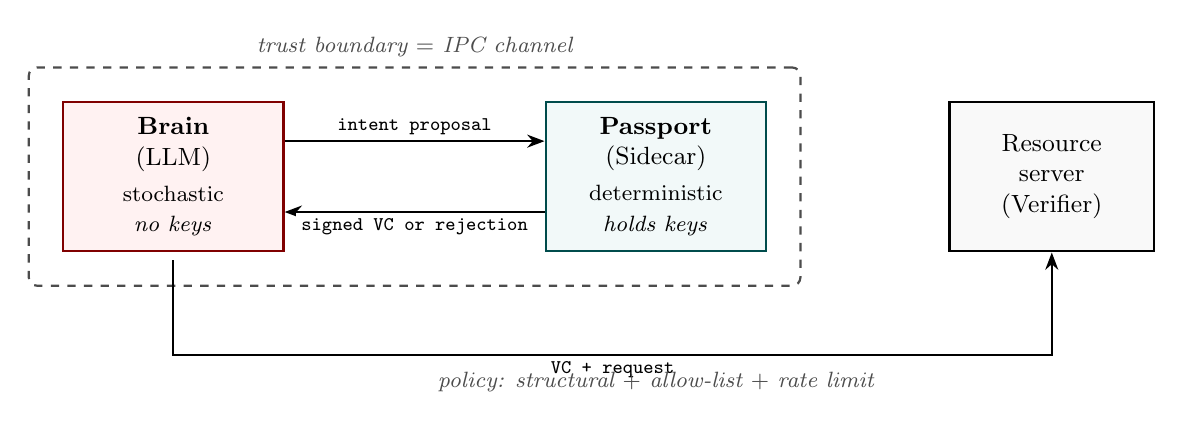
\begin{tikzpicture}[
    box/.style={draw, thick, minimum width=2.8cm, minimum height=1.9cm, align=center, font=\small},
    brain/.style={box, fill=red!5, draw=red!50!black},
    passport/.style={box, fill=teal!5, draw=teal!60!black},
    resource/.style={draw, thick, fill=gray!5, minimum width=2.6cm, minimum height=1.9cm, align=center, font=\small},
    arr/.style={-{Stealth[length=2.2mm]}, thick},
    boundary/.style={draw, dashed, thick, gray!60!black, rounded corners=3pt, inner sep=12pt},
    lbl/.style={font=\footnotesize\itshape, text=gray!60!black, align=center},
    annot/.style={font=\scriptsize\ttfamily, fill=white, inner sep=2pt}
]
% Brain on the left
\node[brain] (brain) at (0, 0) {\textbf{Brain}\\(LLM)\\[2pt]\footnotesize stochastic\\\footnotesize \emph{no keys}};
% Passport in the middle, with extra horizontal gap so arrow labels fit
\node[passport, right=3.3cm of brain] (passport) {\textbf{Passport}\\(Sidecar)\\[2pt]\footnotesize deterministic\\\footnotesize \emph{holds keys}};
% Trust boundary around Brain + Passport
\begin{scope}[on background layer]
  \node[boundary, fit=(brain) (passport), label={[lbl,anchor=south]above:trust boundary $=$ IPC channel}] {};
\end{scope}
% Intent proposal (top arrow Brain -> Passport)
\draw[arr] ($(brain.east) + (0, 0.45)$) -- node[annot, above]{intent proposal} ($(passport.west) + (0, 0.45)$);
% Credential or rejection (bottom arrow Passport -> Brain)
\draw[arr] ($(passport.west) + (0, -0.45)$) -- node[annot, below]{signed VC or rejection} ($(brain.east) + (0, -0.45)$);
% Resource server far right, separate row to avoid arrow clutter
\node[resource, right=2.3cm of passport] (rs) {Resource\\server\\(Verifier)};
% VC + request arrow goes Brain -> below the trust boundary -> RS
\draw[arr] (brain.south) ++ (0, -0.1) -- ++(0, -1.2) coordinate (b1) -| node[annot, pos=0.25, below]{VC + request} (rs.south);
% Allow-list call-out below the Passport, well clear of the boundary
\node[lbl, below=1.4cm of passport] {policy: structural $+$ allow-list $+$ rate limit};
\end{tikzpicture}
\caption{Identity Sidecar pattern. The Brain (LLM) holds no cryptographic secrets and proposes intents over a local IPC channel. The Passport applies a deterministic allow-list policy and signs only intents that pass. A compromised Brain cannot exceed the Passport's enforced scope.}
\label{fig:sidecar}
\end{figure}

\subsection{Just-In-Time Signing Flow}

A signing operation proceeds:

\begin{enumerate}[label=\arabic*.,leftmargin=*]
\item The Brain decides an action is appropriate. It constructs a proposed intent.
\item The Brain submits the intent to the Sidecar over IPC.
\item The Sidecar applies its policy: structural validation (required fields present), allow-list check (action type is in the deployed allow-list), and rate-limit check.
\item If policy passes, the Sidecar constructs the full credential, signs it with the held private key, and returns the credential to the Brain.
\item If policy fails, the Sidecar returns a structured error (\S\ref{sec:sidecar-errors}). No credential is produced.
\end{enumerate}

\subsection{Sidecar Rejection Codes}
\label{sec:sidecar-errors}

When the Sidecar rejects an intent proposal, the response includes a machine-readable \verb|code| and a short remediation hint the Brain can act on:

\begin{itemize}[leftmargin=*,nosep]
\item \verb|intent_action_not_in_allowlist|: the proposed \verb|action| is not configured. Hint: choose from the deployment's allow-list, sample shown in the response.
\item \verb|intent_target_pattern_violation|: the \verb|target| does not match the action's permitted pattern. Hint: regex shown.
\item \verb|intent_resource_out_of_scope|: the \verb|resource| URI is outside the agent's deployed scope. Hint: scope shown.
\item \verb|intent_missing_required_field|: a structural field (\verb|action|, \verb|target|, \verb|resource|) is empty or absent.
\item \verb|rate_limit_exceeded|: the agent has exceeded its per-window signing rate. Hint: retry-after seconds.
\item \verb|delegation_chain_invalid|: when signing a delegation link, the parent chain failed verification. Hint: which link failed and why.
\end{itemize}

Each code is stable across implementations; cross-language contract tests assert the same code is returned for the same failure across Python, TypeScript, and Go sidecars.

The Sidecar's policy check is the last line of defence against a compromised Brain. A prompt-injected LLM can propose any intent it wants; if the intent is not in the allow-list, the Sidecar refuses to sign and returns one of the structured rejection codes in \S\ref{sec:sidecar-errors}. What bounds a compromised Brain is therefore a small daemon's policy file, not the LLM's behaviour or training. Even an attacker with full control of the Brain's context can only get intents signed that the operator already approved as a class.

\subsection{Reference Implementations and Tier Hierarchy}

Three reference Sidecar implementations ship with the protocol. All three speak the same HTTP wire contract (the byte-level request and response shapes a Sidecar must produce and accept) and accept/reject the same inputs, enforced by a shared contract test suite. Tier guidance:

\begin{table}[h]
\centering
\footnotesize
\renewcommand{\arraystretch}{1.15}
\begin{tabularx}{\textwidth}{@{}l Y l@{}}
\toprule
\textbf{Implementation} & \textbf{Capabilities} & \textbf{Target tier} \\
\midrule
\verb|go-sidecar/| (Go)            & KMS/HSM, dual-proof PQ, JWE wrapping, multi-tenant & Production / regulated \\
\verb|vouch.sidecar.*| (Python)    & File or env keys; omits KMS, PQ, JWE, multi-tenancy & Self-hosted, dev \\
\verb|packages/sdk-ts/sidecar/| (TS) & Same scope as Python                              & Node stacks \\
\bottomrule
\end{tabularx}
\end{table}

% ====================================================================
\section{Delegation Chains}
\label{sec:delegation}

\subsection{Motivation}

Multi-agent systems present an attribution problem: an action taken by a leaf agent may have been authorized by a chain of principals: a user authorized an assistant, which authorized a research agent, which authorized a web-scraping sub-agent. When the action requires audit, the leaf-only signing model loses the chain.

Vouch delegations are themselves Verifiable Credentials. Each link in a chain is a credential signed by the delegating principal and identifying the delegate. A leaf-action credential includes the full chain (or a reference to it) so a verifier can reconstruct the authorization path from root principal to leaf agent.

\subsection{Delegation Link Structure}

A delegation link is a signed object (a Vouch credential carrying delegation fields) shaped:

\begin{lstlisting}[language=json]
{
  "issuer": "did:web:assistant.example.com",
  "subject": "did:web:research-agent.example.com",
  "intent": {
    "action": "web_search",
    "target": "topic:climate-2026",
    "resource": "https://research-agent.example.com/agents/research-agent/scope/2026"
  },
  "validFrom": "2026-05-14T06:00:00Z",
  "validUntil": "2026-05-14T08:00:00Z",
  "proof": { "...DataIntegrityProof..." }
}
\end{lstlisting}

The link's \verb|issuer| is the delegating principal; \verb|subject| is the delegate. The \verb|intent| object (\verb|action|, \verb|target|, \verb|resource|) describes the authorized action and the resource URI under which it must fall; \verb|validFrom| and \verb|validUntil| bound the delegation in time. Each link is signed by its \verb|issuer|.

\subsection{Chain Construction, Narrowing, and Depth}

A chain is a list of delegation-link credentials, ordered from root principal to leaf agent. At each link, the child's \verb|intent.resource| MUST be the same as, or a sub-URI of, the parent's \verb|intent.resource| (the \emph{narrowing rule}). The rule is one-directional: a delegate may pass its full scope down unchanged, or pass a narrower subset, but never broaden. Equal scope is permitted (a wrapper agent that does not specialize beyond its parent); strictly broader scope is the violation that triggers \verb|scope_exceeds_parent|. Chain depth is bounded to \textbf{five links maximum}, which prevents pathological chains from inflating verification cost or obscuring the actual authorization path.

\begin{figure}[h]
\centering
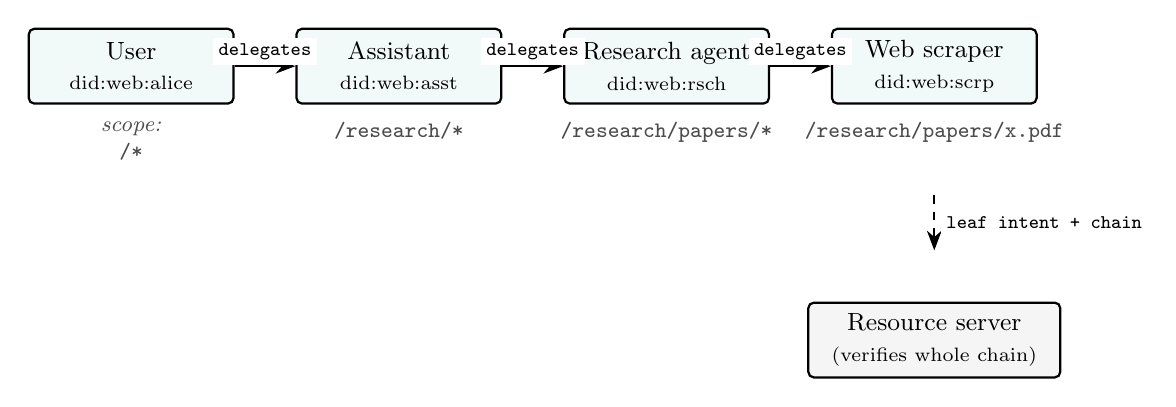
\begin{tikzpicture}[
    principal/.style={draw, thick, rounded corners=2pt, fill=teal!5, minimum width=2.6cm, minimum height=0.95cm, align=center, font=\small},
    link/.style={font=\scriptsize\ttfamily, align=center, fill=white, inner sep=2pt},
    arr/.style={-{Stealth[length=2.5mm]}, thick},
    annot/.style={font=\footnotesize\itshape, text=gray!60!black, align=center}
]
% Principals
\node[principal] (user)   at (0, 0)   {User\\\scriptsize did:web:alice};
\node[principal] (asst)   at (3.4, 0) {Assistant\\\scriptsize did:web:asst};
\node[principal] (res)    at (6.8, 0) {Research agent\\\scriptsize did:web:rsch};
\node[principal] (leaf)   at (10.2, 0){Web scraper\\\scriptsize did:web:scrp};
% Delegation links
\draw[arr] (user)   -- node[link, above]{delegates}     (asst);
\draw[arr] (asst)   -- node[link, above]{delegates}     (res);
\draw[arr] (res)    -- node[link, above]{delegates}     (leaf);
% Scope narrows
\node[annot, below=0.1cm of user]   {scope:\\\verb|/*|};
\node[annot, below=0.1cm of asst]   {\verb|/research/*|};
\node[annot, below=0.1cm of res]    {\verb|/research/papers/*|};
\node[annot, below=0.1cm of leaf]   {\verb|/research/papers/x.pdf|};
% Action arrow downward from leaf
\draw[arr, dashed] (leaf.south) ++ (0, -1.15) -- node[link, right, xshift=2pt]{leaf intent + chain}+(0, -0.7);
\node[principal, fill=gray!8, below=2.5cm of leaf, minimum width=3.2cm] (rs){Resource server\\\scriptsize (verifies whole chain)};
\end{tikzpicture}
\caption{Delegation chain. Each link records the parent's DID (\texttt{issuer}), the child's DID (\texttt{subject}), the intent handed down (action, target, resource), and a Data Integrity proof. Scope narrows at each link in this example, but equal scope between adjacent links is also permitted; only strict broadening triggers \texttt{scope\_exceeds\_parent}. The resource server validates the entire chain on every request: signatures, narrowing, depth limit, and the leaf intent's action against the deepest link's allow-list.}
\label{fig:delegation}
\end{figure}

\subsection{Chain Validation}

A verifier validating a leaf credential with an attached chain:

\begin{enumerate}[label=\arabic*.,leftmargin=*]
\item Verifies the leaf credential's signature.
\item Walks the chain from the leaf link back to the root.
\item For each adjacent pair, verifies that the parent link's \verb|subject| equals the child link's \verb|issuer|.
\item Verifies the root link's \verb|issuer| is in the verifier's set of trusted principals.
\item For each link, verifies its \verb|intent.resource| is the same as, or a sub-URI of, the parent link's \verb|intent.resource| (the narrowing rule).
\item For each link, verifies its \verb|validFrom|/\verb|validUntil| fall within the parent link's temporal bounds.
\item Verifies each link's Data Integrity proof.
\end{enumerate}

Any failure produces a structured rejection reason. The protocol defines six:

\begin{itemize}[leftmargin=*,nosep]
\item \verb|untrusted_principal|: the root link's issuer is not in the verifier's trust set.
\item \verb|chain_depth_exceeded|: the chain length exceeds the configured maximum.
\item \verb|scope_exceeds_parent|: a link's \verb|intent.resource| is broader than its parent's (equal scope is permitted; only strict broadening is the violation).
\item \verb|temporal_bounds_exceeded|: a link's validity window falls outside its parent's.
\item \verb|subject_issuer_mismatch|: a link's \verb|subject| does not match the next link's \verb|issuer|.
\item \verb|link_signature_invalid|: a link's Data Integrity proof fails.
\end{itemize}

% ====================================================================
\section{Revocation}
\label{sec:revocation}

\subsection{Two Mechanisms}

Vouch supports two complementary revocation mechanisms:

\begin{itemize}[leftmargin=*]
\item \textbf{DID-level revocation}: revoke an entire DID, invalidating all credentials it has issued or ever will issue.
\item \textbf{Credential-level revocation}: revoke a specific credential without affecting other credentials from the same issuer.
\end{itemize}

Most production deployments run both. DID-level revocation is appropriate for blanket kill switches (key compromise, agent decommissioning); credential-level revocation is appropriate for surgical retraction (regulatory hold on a specific transaction, suspension pending review).

\subsection{DID-Level Revocation Registry}

The protocol defines a revocation registry interface (\verb|RevocationStoreInterface|). A revoked DID is recorded as a \verb|RevocationRecord| with \verb|did|, \verb|revoked_at|, \verb|reason|, and \verb|revoked_by|. Reference implementations include in-memory, file, and Redis backends.

Verifiers consult the registry on every credential verification. If the issuing DID is in the registry, the credential is rejected with \verb|issuer_revoked|. The registry's cache TTL is operator-configurable; a typical default is 60 seconds.

\subsection{BitstringStatusList for Per-Credential Revocation}

For per-credential revocation, Vouch uses W3C BitstringStatusList~\cite{w3cbsl}. The issuer maintains a published \texttt{BitstringStatusListCredential} whose \verb|credentialSubject.encodedList| is a gzip-compressed, base64url-encoded bitstring. Each Vouch credential includes a \verb|credentialStatus| property pointing at its index. A verifier fetches the status list, decompresses, reads the indicated bit; if the bit is set, the credential is revoked.

The protocol's \verb|StatusListFetcher| caches the status list with a configurable TTL and supports conditional GETs (\verb|If-None-Match|, \verb|If-Modified-Since|) for efficient re-validation.

% ====================================================================
\section{Dual-Proof Post-Quantum Profile}
\label{sec:hybrid}

\subsection{Motivation}

NIST's selection of ML-DSA-44 (FIPS 204) as a standardized post-quantum digital signature~\cite{nistfips204} places a known cryptographic transition on the protocol's horizon. Ed25519 will not survive a sufficiently large fault-tolerant quantum computer. The transition window is uncertain but real, and credentials with multi-year audit retention requirements (regulated healthcare, financial settlement) cannot afford to be signed with an algorithm that will be broken before the retention window expires.

The protocol's response is the \emph{dual-proof profile}: a credential carries two independent W3C Data Integrity proofs on the same JCS-canonicalized credential bytes, one \texttt{eddsa-jcs-2022} proof (classical Ed25519) and one \texttt{mldsa44-jcs-2026} proof (ML-DSA-44). The Data Integrity specification already defines the \verb|proof| field as an array, so the dual-proof construction is a natural use of existing primitives and requires no Vouch-specific composite cryptosuite identifier.

\subsection{Construction}

The credential's \verb|proof| field is an array of two Data Integrity proof objects:

\begin{verbatim}
"proof": [
  {
    "type": "DataIntegrityProof",
    "cryptosuite": "eddsa-jcs-2022",
    "verificationMethod": "...#key-ed25519",
    "proofPurpose": "assertionMethod",
    "proofValue": "z<base58btc(ed25519_sig)>"
  },
  {
    "type": "DataIntegrityProof",
    "cryptosuite": "mldsa44-jcs-2026",
    "verificationMethod": "...#key-mldsa44",
    "proofPurpose": "assertionMethod",
    "proofValue": "z<base58btc(mldsa44_sig)>"
  }
]
\end{verbatim}

Both proofs are computed over the same JCS-canonical credential bytes (the credential minus the \verb|proofValue| field of each proof, JCS-canonicalized). The same-canonical-bytes property is preserved by construction: both cryptosuites use JCS canonicalization on the same credential body. Each proof's \verb|proofValue| is independently multibase base58btc-encoded.

The Ed25519 signature is exactly 64 bytes; the ML-DSA-44 signature is exactly 2,420 bytes. Each appears in its own proof object's \verb|proofValue| rather than being concatenated into a single field.

\subsection{Verifier Modes}

A verifier iterates the credential's \verb|proof| array and applies one of three local policies:

\begin{enumerate}[label=\arabic*.,leftmargin=*]
\item \textbf{Classical-only}: validate the \texttt{eddsa-jcs-2022} proof; ignore the rest. Useful when ML-DSA-44 libraries are unavailable or computationally expensive.
\item \textbf{Post-quantum-only}: validate the \texttt{mldsa44-jcs-2026} proof. Useful when classical signatures are no longer trusted under the verifier's compliance regime.
\item \textbf{Both-required}: validate every proof in the array; reject if any one fails. The cautious mode, recommended for long-retention credentials.
\end{enumerate}

The verifier's mode is policy, not part of the credential. The same credential is verifiable under any verifier mode without re-signing.

\subsection{DID Document Representation}

A signing DID supporting the dual-proof profile publishes two verification methods in its DID Document: one Ed25519 Multikey, one ML-DSA-44 Multikey. The Multikey multicodec prefix distinguishes the two algorithms, and each proof's \verb|verificationMethod| field points at its own key.

\subsection{Migration Path}

A deployment migrates from classical to dual-proof in three steps:

\begin{enumerate}[label=\arabic*.,leftmargin=*]
\item \textbf{Adopt dual-proof signing}: the signer issues credentials with two proofs in the array. Existing classical-only verifiers continue working (they see a familiar \texttt{eddsa-jcs-2022} proof and ignore the second one they don't recognize).
\item \textbf{Update verifiers}: deploy a verifier release that supports ML-DSA-44. Configure the verifier's mode (classical-only, PQ-only, or both-required) based on the deployment's risk tolerance.
\item \textbf{Retire classical signing}: once all verifiers are PQ-aware, switch the signer to issue only the \texttt{mldsa44-jcs-2026} proof. The dual-proof profile is the migration vehicle, not the destination.
\end{enumerate}

\subsection{Relationship to Concurrent Work}

The dual-proof construction converges with Digital Bazaar's \texttt{mldsa44-rdfc-2024-cryptosuite} family~\cite{db-mldsa44}, which defines an ML-DSA-44 Data Integrity cryptosuite using RDFC canonicalization, and with that family's forthcoming JCS variant. The cryptosuite identifier \texttt{mldsa44-jcs-2026} used in this paper is provisional and is being aligned with that upstream registration. Earlier Vouch reference implementations (v1.6.x) emit a single composite cryptosuite (\texttt{hybrid-eddsa-mldsa44-jcs-2026}) with a concatenated \verb|proofValue|; this composite identifier is retained as a transitional alias for backward compatibility only, and new implementations emit the dual-proof form described above.

% ====================================================================
\section{The State Verifiability Layer}
\label{sec:state}

\subsection{Motivation: From Point-in-Time to Continuous}

The credential layer addresses ``did the agent claim authorization at time $T$.'' The State Verifiability layer addresses operational questions arising \emph{after} that: is the agent still behaving correctly \emph{now}? Has it drifted out of policy? Has it been substituted? Has it crashed silently and been replayed by an adversary?

A long-running agent without continuous attestation accumulates risk. The longer it runs, the wider the window during which a compromise or substitution may go undetected. Heartbeat-style renewal makes that window bounded.

\paragraph{What this layer costs.} The five mechanisms (heartbeat, decay, behavioural attestation, canary, Merkle root) together add roughly one validator round trip per heartbeat interval (typically 60 seconds), $\leq 1$ KB of state per agent on the validator, and a 30--50\,ms verification cost on the agent side per heartbeat. Per-action overhead (the cost the resource server pays when checking an admitted credential against the current voucher) is sub-millisecond (one decay computation plus a threshold comparison). Section~\ref{sec:eval} reports the numbers in detail. The layer is opt-in at the protocol level: agents that only sign occasional actions, with no long-running runtime, can omit State Verifiability entirely and ship only the credential layer.

\subsection{The Heartbeat Protocol}

The Heartbeat Protocol defines a periodic renewal cycle:

\begin{enumerate}[label=\arabic*.,leftmargin=*]
\item The agent's \verb|HeartbeatSession| records actions and behavioural signals during each interval.
\item At the heartbeat boundary (default 60 seconds), the session constructs a \verb|HeartbeatRequest|: it includes a behavioural digest, the running Merkle root of actions performed since the last heartbeat, the canary commit/reveal pair, and an interval index.
\item The agent submits the request to a validator (or quorum of validators).
\item The validator(s) check schema, behavioural digest structure, canary chain integrity, interval-index monotonicity, and trust policy.
\item On success, the validator returns a fresh \verb|SessionVoucher|: itself a Vouch Credential under the validator's DID, whose \verb|credentialSubject| carries the renewed \texttt{initialTrust} and \texttt{decayLambda} parameters for the agent.
\item On failure (broken canary, stale interval index, behavioural drift), no SessionVoucher is issued, the agent's existing one expires within seconds (Definition~\ref{def:trust-decay}), and the resource server denies any subsequent action whose trust threshold $\theta_a$ exceeds the now-decayed trust (Definition~\ref{def:admissibility}). The agent does not need to be ``told'' it has lost authority: the next time it presents a credential to a resource server, the server checks the SessionVoucher's age against $\lambda$ and refuses if $T(t) < \theta_a$. The heartbeat interval is a configurable parameter (default 60\,s, minimum 5\,s, maximum bounded by the chosen $\lambda$ so that renewal stays ahead of decay; \S\ref{sec:trust-decay}).
\end{enumerate}

The Heartbeat Protocol inverts the traditional PKI trust model from ``trusted until revoked'' to \emph{``untrusted until renewed.''}

\begin{figure}[h]
\centering
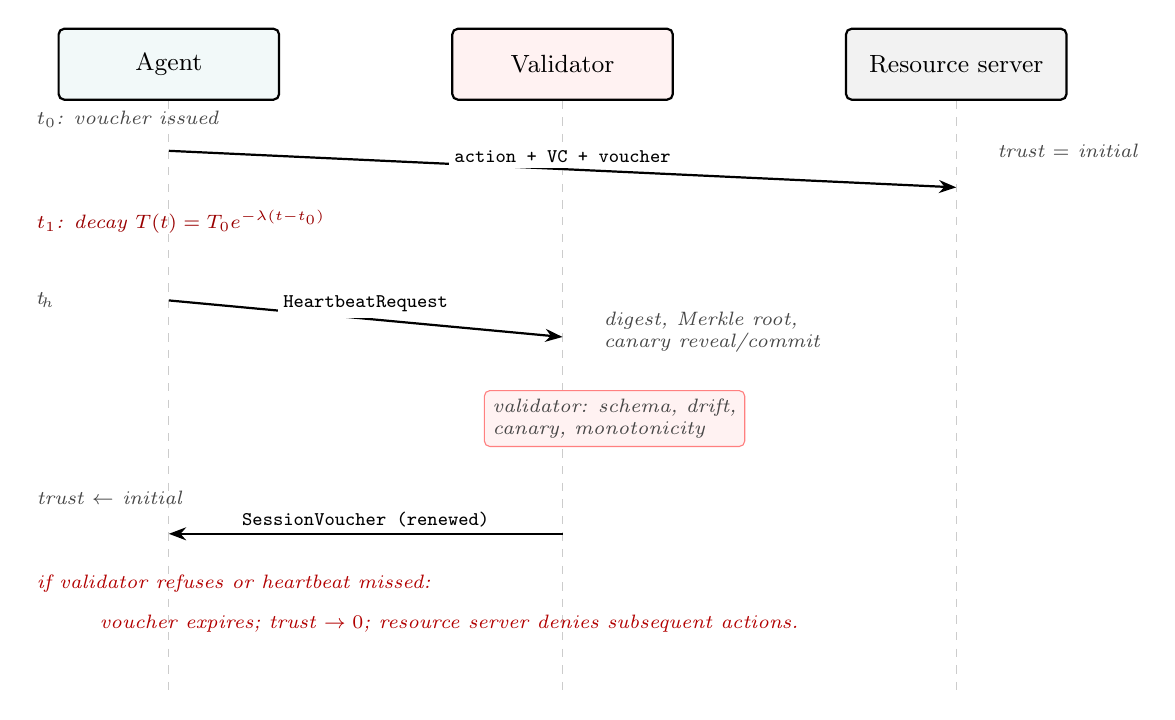
\begin{tikzpicture}[
    node distance=0.6cm and 0.8cm,
    agentbox/.style={draw, thick, rounded corners=2pt, fill=teal!5, minimum width=2.8cm, minimum height=0.9cm, align=center, font=\small},
    valbox/.style={draw, thick, rounded corners=2pt, fill=red!5, minimum width=2.8cm, minimum height=0.9cm, align=center, font=\small},
    rsbox/.style={draw, thick, rounded corners=2pt, fill=gray!10, minimum width=2.8cm, minimum height=0.9cm, align=center, font=\small},
    arr/.style={-{Stealth[length=2.2mm]}, thick},
    msg/.style={font=\scriptsize\ttfamily, fill=white, inner sep=2pt},
    annot/.style={font=\scriptsize\itshape, text=gray!55!black, align=left}
]
% Lifelines
\node[agentbox] (a0) at (0, 0) {Agent};
\node[valbox]   (v0) at (5, 0) {Validator};
\node[rsbox]    (r0) at (10, 0){Resource server};
% Vertical lifelines
\draw[gray!40, dashed] (a0.south) -- ++(0, -7.5);
\draw[gray!40, dashed] (v0.south) -- ++(0, -7.5);
\draw[gray!40, dashed] (r0.south) -- ++(0, -7.5);
% --- Interval 1: action ---
\node[annot, anchor=west] at (-1.8, -0.7) {$t_0$: voucher issued};
\draw[arr] (a0.south |- 0, -1.1) -- node[msg, above]{action + VC + voucher} ($(r0.south) + (0, -1.1)$);
\node[annot, anchor=west] at (10.4, -1.1) {trust $=$ initial};
% --- Decay arrow ---
\node[annot, anchor=west, text=red!60!black] at (-1.8, -2.0) {$t_1$: decay $T(t)=T_0 e^{-\lambda(t-t_0)}$};
% --- Heartbeat boundary ---
\draw[arr] (a0.south |- 0, -3.0) -- node[msg, above]{HeartbeatRequest} ($(v0.south) + (0, -3.0)$);
\node[annot, anchor=west] at (-1.8, -3.0) {$t_{\!h}$};
\node[annot, anchor=west] at (5.4, -3.4) {digest, Merkle root,\\canary reveal/commit};
% --- Validator check ---
\node[annot, anchor=west, fill=red!5, draw=red!50, rounded corners=2pt, inner sep=3pt] at (4.0, -4.5) {validator: schema, drift,\\canary, monotonicity};
% --- New voucher ---
\draw[arr] ($(v0.south) + (0, -5.5)$) -- node[msg, above]{SessionVoucher (renewed)} ($(a0.south) + (0, -5.5)$);
\node[annot, anchor=west] at (-1.8, -5.5) {trust $\leftarrow$ initial};
% --- Failure branch ---
\node[annot, anchor=west, text=red!70!black] at (-1.8, -6.6) {if validator refuses or heartbeat missed:};
\node[annot, anchor=west, text=red!70!black] at (-1.0, -7.1) {voucher expires; trust $\to 0$; resource server denies subsequent actions.};
\end{tikzpicture}
\caption{Heartbeat lifecycle. Each interval the agent's voucher trust decays exponentially. At the heartbeat boundary the agent submits a digest, an action Merkle root, and a canary commit/reveal to the validator. A renewed voucher resets trust. A missed or rejected heartbeat lets the existing voucher expire, and trust drives below the action's threshold within seconds.}
\label{fig:heartbeat}
\end{figure}

\subsection{Trust Entropy Decay}
\label{sec:trust-decay}

Each SessionVoucher carries two scalars: an initial trust value $T_0 \in (0, 1]$ (the \texttt{initialTrust} field) and a decay rate $\lambda > 0$ (the \texttt{decayLambda} field).

\begin{definition}[Trust entropy decay]\label{def:trust-decay}
Let $t_0$ be the timestamp at which a validator (or quorum) issued the SessionVoucher. The voucher's \emph{effective trust} at any time $t \geq t_0$ is
\[
T(t) \;=\; T_0 \cdot e^{-\lambda (t - t_0)}
\]
with $T(t_0) = T_0$ and $\lim_{t \to \infty} T(t) = 0$. The voucher's \emph{half-life} is $\tau_{1/2} = \ln(2)/\lambda$.
\end{definition}

\begin{definition}[Action admissibility]\label{def:admissibility}
For an action $a$ with associated risk threshold $\theta_a \in (0, 1]$, the resource server admits the request only if
\[
T(t_{\text{verify}}) \;\geq\; \theta_a
\]
where $t_{\text{verify}}$ is the timestamp at which the resource server evaluates the request. Equivalently, the voucher's \emph{admissibility window} for action $a$ is bounded above by
\[
\Delta_a \;=\; \frac{1}{\lambda}\ln\!\left(\frac{T_0}{\theta_a}\right).
\]
\end{definition}

\begin{definition}[Adversary capability bound]\label{def:adversary}
Let $\mathcal{A}$ denote an adversary that has compromised the agent's Brain (LLM context) but not its Passport (signing process). Let $a^\star$ be any action with $\theta_{a^\star} > 0$ outside the deployed allow-list of the Passport. Then for all $t \geq t_0$:
\[
\Pr\!\left[\mathcal{A} \text{ obtains a valid VC for } a^\star\right] \;\leq\; \Pr\!\left[\text{Ed25519 forgery}\right] + \Pr\!\left[\text{Passport compromise} \mid \mathcal{A}\right],
\]
i.e., the adversary's success probability is bounded by the underlying signature-scheme assumption plus a separate compromise of the Passport, independent of how the Brain misbehaves. The Sidecar's allow-list converts the security argument from ``trust the LLM not to be prompt-injected'' into ``trust that a small, audited, deterministic policy daemon is not compromised.''
\end{definition}

Sensitive actions are gated by current trust. The specification defines five reference thresholds by operation category:

\begin{itemize}[leftmargin=*]
\item Financial transaction: $\theta = 0.95$ (transfers, settlement, regulated submissions).
\item API write: $\theta = 0.80$ (state-changing calls, code deployment).
\item API read: $\theta = 0.50$ (PHI read, customer-data access, status queries).
\item Health check: $\theta = 0.20$ (liveness, idle activity).
\item Logging: $\theta = 0.05$ (telemetry, audit emission).
\end{itemize}

Heartbeat interval should be set to less than half the half-life so renewal stays ahead of decay. For $\lambda = 0.01$, half-life is approximately 69 seconds; a 30-second heartbeat is appropriate.

\paragraph{Worked example.} Suppose an agent is issued a voucher at $t_0 = 0$ with $T_0 = 1.0$ and $\lambda = 0.01\,\text{s}^{-1}$ (half-life $\approx 69$\,s). The agent attempts a financial transfer at $t = 90$\,s ($\theta = 0.95$). Compute $T(90) = 1.0 \cdot e^{-0.01 \cdot 90} = 0.407$. Since $0.407 < 0.95$, the resource server denies. The agent must heartbeat first; if it does so at $t = 25$\,s and is renewed, then at $t = 90$\,s the post-renewal effective age is $90 - 25 = 65$\,s, giving $T(90) = e^{-0.65} = 0.522$, still below $0.95$. To remain admissible for $\theta = 0.95$, the agent must heartbeat at most $\Delta_{0.95} = (1/0.01)\ln(1/0.95) \approx 5.1$\,s before each financial action. The same agent's API-read actions ($\theta = 0.50$) tolerate $\Delta_{0.50} \approx 69$\,s. Different thresholds, same voucher.

\subsection{Behavioural Attestation}

Per-interval, the \verb|BehavioralCollector| records:

\begin{itemize}[leftmargin=*]
\item API calls made by the agent (URL, token count, optional intent-drift score)
\item Resources accessed
\item Any policy-defined custom signals
\end{itemize}

At each heartbeat, the collector produces a \verb|behavioralDigest|. Three reference intent-drift scorers ship with the SDK: arithmetic mean, maximum-of-samples, and exponential-weighted moving average. The drift score quantifies the divergence of the agent's recent activity from a baseline; a sharp rise across consecutive intervals signals a potential prompt-injection or policy-drift event.

The v0.1 scorers measure \emph{statistical} drift (URL distribution, action mix, request rate) rather than \emph{semantic} alignment with the original approved intent. Closing that gap (inferring whether a 60-second interval's micro-actions are still on the path to the principal's stated end goal) requires an LLM-judge step that is outside the Sidecar's deterministic boundary and is therefore left to a follow-up specification. Until then, behavioural drift is a coarse alarm; deployments with strict semantic-alignment requirements should pair Vouch with their own per-action policy validator.

\subsection{Canary Commitments}

The canary commit/reveal chain provides cryptographic detection of silent agent failure. Each heartbeat commits to a fresh 256-bit secret hash; the next heartbeat reveals the prior secret. A missed heartbeat means the prior secret is never revealed; no subsequent heartbeat can resume the chain because the validator expects the missing reveal.

The validator state per agent is one string (the last commitment). The state is cheap to persist and survives validator restarts.

\subsection{Action Merkle Roots}

A \verb|HeartbeatRequest| includes the Merkle root of actions performed since the last heartbeat, computed over RFC 6962-domain-separated Merkle trees~\cite{rfc6962}. Each action is hashed with \texttt{0x00} prefix (leaf); internal nodes are hashed with \texttt{0x01} prefix. The domain separation prevents the classical second-preimage attack on Merkle trees. In practice, the root commits the agent to its full action history for the interval: any later auditor (the resource server, a regulator, the principal who delegated) can demand the agent disclose the leaves and verify that what it discloses matches the root the validator signed. The agent cannot quietly drop actions, reorder them, or swap one for another without breaking the root: the validator's signature is the cryptographic anchor.

\subsection{Validator Quorum}

Single validators are single points of failure. The \verb|HeartbeatQuorum| distributes trust evaluation across multiple validators with different responsibilities:

\begin{lstlisting}[language=Python]
quorum = HeartbeatQuorum(
    validators=[
        QuorumValidator(validator=policy_validator,     role=ROLE_POLICY),
        QuorumValidator(validator=behavioral_validator, role=ROLE_BEHAVIORAL),
        QuorumValidator(validator=budget_validator,     role=ROLE_BUDGET),
    ],
    threshold=2,
)
\end{lstlisting}

Roles are reference tags; deployments choose their own role taxonomy. The quorum threshold is $M$-of-$N$. Trust parameter aggregation across approving validators is configurable; the defaults bias toward caution.

% ====================================================================
\section{Security Analysis}
\label{sec:security}

\subsection{Threat Model}

The protocol assumes:

\begin{itemize}[leftmargin=*]
\item The cryptographic primitives (Ed25519, ML-DSA-44, SHA-256) are sound under their respective security assumptions.
\item The verifier can resolve the issuer's DID Document via the agent's chosen DID method (\texttt{did:web} via HTTPS, \texttt{did:key} via decoding).
\item The verifier has access to the revocation registry and to BitstringStatusList endpoints.
\item The Identity Sidecar's process boundary is enforced by the host operating system: a malicious LLM process cannot read the Sidecar's memory.
\end{itemize}

The protocol does \emph{not} assume:

\begin{itemize}[leftmargin=*]
\item The LLM is trustworthy. Prompt injection, jailbreak, and model substitution attacks are within the threat model.
\item The transport layer is confidential. Credentials are designed to be exposed in transit (the signature establishes authenticity even when an adversary observes the credential).
\item The agent's host platform is uncompromised. Root-level compromise of the host defeats any application-level defence, including this one.
\end{itemize}

\subsection{Defended Threats}

\noindent\textbf{Bearer-credential theft.} Vouch credentials are bound to the issuer's DID by signature; an adversary who copies a credential cannot reuse it to issue new credentials. The original credential is bound to its \verb|intent.target| and \verb|intent.resource|; it cannot be replayed against a different resource.

\noindent\textbf{Prompt injection causing key exfiltration.} The Identity Sidecar makes this attack class structurally impossible: the LLM process has no access to the private key.

\noindent\textbf{Prompt injection causing unauthorized credential issuance.} The Sidecar's intent allow-list makes this attack class capability-bounded. The check is a deterministic string-and-pattern comparison run inside the Sidecar process: the proposed \verb|intent.action| is looked up in the configured allow-list dictionary, the \verb|intent.target| is matched against the action's permitted regex, and the \verb|intent.resource| is checked to fall under the agent's deployed scope URI. None of these decisions involve the LLM. A prompt-injected Brain that proposes a previously-unknown action receives \verb|intent_action_not_in_allowlist|; an injection that tries to widen an existing action's target receives \verb|intent_target_pattern_violation|. Both responses are signed by the Sidecar but contain no credential the agent can present to a resource server.

\noindent\textbf{Replay across resources.} Each credential's \verb|intent.resource| is part of the signed payload. Replaying against a different resource invalidates the signature.

\noindent\textbf{Delegation chain forgery.} Each link is a signed credential; forging a link requires possessing the delegating principal's key. Principal anchoring ensures the chain root is known to the verifier independently: the verifier holds (or resolves through DNS) the public key of its accepted root principals and refuses any chain whose root is not in that set.

\noindent\textbf{Scope widening across a chain.} The verifier walks the chain pairwise (parent, child) and computes whether the child's \verb|intent.resource| is a prefix of (or equal to) the parent's, using normal URI prefix matching (path-component-wise after canonicalization). It also checks that each link's validity window falls within its parent's. Either check failing produces \verb|scope_exceeds_parent| (or \verb|temporal_bounds_exceeded|); the chain is rejected before any credential is admitted.

\noindent\textbf{Resource widening at delegation.} The chain validator's resource-narrowing rule rejects chains where any link grants access beyond its parent's scope.

\noindent\textbf{Long-running agent silent failure.} The Heartbeat Protocol's canary chain detects missed heartbeats: the next heartbeat cannot produce the expected reveal, the chain breaks, and the validator refuses to renew.

\noindent\textbf{Key compromise.} DID-level revocation invalidates all credentials issued by the compromised key. Resource servers learn of the revocation through one of two mechanisms in the spec: (i) BitstringStatusList polling on a configured interval (typically 60--300\,s), or (ii) the DID Document's revocation marker, which is fetched at credential-verification time alongside the DID Document. A revoked DID's credentials begin failing at the next status-list fetch or DID resolution, whichever comes first. The auto-rotation pipeline automates rotation when leak detection fires; the new DID Document and BitstringStatusList update are published together so verifiers transition without a window during which both keys are valid.

\noindent\textbf{Post-quantum cryptanalysis.} The dual-proof profile carries an ML-DSA-44 Data Integrity proof in addition to the Ed25519 proof, allowing the credential to be re-verified against the PQ proof once Ed25519 is broken. Verifiers in both-required mode are immune to single-algorithm cryptanalysis.

\subsection{Residual Threats}

\noindent\textbf{Within-allow-list abuse.} The Sidecar's allow-list bounds capability \emph{type}, not \emph{abuse within type}. Mitigations: pattern strictness, rate limits, downstream verifier policy, and human-in-the-loop confirmation for ambiguous cases.

\noindent\textbf{DID resolution failures.} If the issuer's DID Document is unreachable, the credential cannot be verified. Verifiers MUST fail closed rather than accept unverified credentials.

\noindent\textbf{Trusted-principal anchor compromise.} If a root principal DID is compromised, the adversary can construct delegation chains rooted at that DID that authorize arbitrary leaf actions within the principal's scope. Defence: rotate root principal keys regularly; require multi-key signing at the root for high-stakes deployments.

% ====================================================================
\section{Cross-Language Interoperability}
\label{sec:interop}

\subsection{Test Vectors}

The protocol ships cross-language test vectors verifying that Python, TypeScript, and Go implementations produce byte-identical credentials given identical inputs:

\begin{itemize}[leftmargin=*]
\item \verb|test-vectors/jcs/|: JSON Canonicalization Scheme reference outputs.
\item \verb|test-vectors/eddsa-jcs-2022/|: full credential signing test vectors for the classical cryptosuite.
\item \verb|test-vectors/hybrid-eddsa-mldsa44/|: full credential signing test vectors for the dual-proof post-quantum profile (and, for v1.6.x interop, the transitional composite cryptosuite).
\item \verb|test-vectors/bitstring-status-list/|: BitstringStatusList encoding test vectors.
\item \verb|test-vectors/sidecar-contract/|: HTTP wire-contract test suite for the three sidecar implementations.
\end{itemize}

\subsection{Reference Implementation Properties}

\begin{table}[h]
\centering
\small
\begin{tabular}{lllrrl}
\toprule
Implementation & Language & LOC & Tests & Cryptosuites & Sidecar tier \\
\midrule
\verb|vouch/| & Python 3.10+ & 4{,}500 & 350 & classical + dual-proof & Lightweight + Dev \\
\verb|packages/sdk-ts/| & TypeScript 5+ & 3{,}200 & 120 & classical + dual-proof & Lightweight \\
\verb|go-sidecar/| & Go 1.21+ & 2{,}800 & 75 & classical + dual-proof & Production \\
\bottomrule
\end{tabular}
\caption{Reference implementations of the Vouch Protocol.}
\end{table}

All three pass the cross-language test vectors. CI runs the vectors on every commit, and rejects merges that introduce divergence.

\subsection{Known Implementation Divergences}

The only documented divergence is in BitstringStatusList byte-encoding: Python and TypeScript use \texttt{zlib}'s DEFLATE encoder, which produces byte-identical output for identical bitstrings; Go's \texttt{compress/flate} produces a valid but different DEFLATE stream. The spec requires equivalence of the \emph{decompressed} bitstring; all three implementations agree on the decompressed bitstring and therefore on every credential's revocation status. Verifiers and issuers interoperate across all three.

% ====================================================================
\section{Expected Performance and Resource Costs}
\label{sec:eval}

This section reports the expected per-operation costs of the protocol. The numbers below are \emph{indicative}: cryptographic-primitive costs (Ed25519, ML-DSA-44, SHA-256) are taken from the well-characterized published benchmarks of the reference implementations (\texttt{libsodium}, \texttt{cryptography}, \texttt{@noble/ed25519}, \texttt{crypto/ed25519}, the NIST FIPS 204 reference implementation~\cite{nistfips204}); protocol-composition costs (JCS canonicalization, multibase encoding, Sidecar IPC, chain validation) are derived from prototype measurements during development and rounded to the appropriate order of magnitude. A reproducible, hardware-pinned benchmark harness ships with the v1.0 release of the reference implementation; the cross-language interoperability follow-up paper will report measured wall-clock medians of $10^4$ runs on documented hardware with confidence intervals. Treat the numbers in this section as design targets, not measured ground truth.

\subsection{Per-Credential Signing and Verification Cost}

\begin{table}[h]
\centering
\small
\begin{tabular}{lrrr}
\toprule
\textbf{Operation} & \textbf{Ed25519} & \textbf{ML-DSA-44} & \textbf{Dual-proof} \\
\midrule
Sign (full credential, JCS + hash + signature) & $\sim$50~\textmu s & $\sim$3~ms & $\sim$3~ms \\
Verify (signature check, DID Document resolved) & $\sim$100~\textmu s & $\sim$1~ms & $\sim$1~ms \\
Verify with delegation chain depth 3 & $\sim$300~\textmu s & $\sim$3~ms & $\sim$3~ms \\
\bottomrule
\end{tabular}
\caption{Indicative signing and verification costs. Ed25519 and ML-DSA-44 numbers are within an order of magnitude of the public benchmarks of \texttt{cryptography} and the NIST FIPS 204 reference implementation; per-credential overhead (JCS canonicalization, multibase encoding) is derived from prototype runs. Dual-proof cost is dominated by ML-DSA-44; Ed25519 adds about 2\%. For per-action signing at $\leq$10 ops/s/agent, dual-proof cost is invisible in end-to-end latency.}
\label{tab:sign-cost}
\end{table}

\subsection{Credential Size and Wire Overhead}

Credential size matters for transport-layer constraints (HTTP header caps, QR code capacity). Table~\ref{tab:size} reports indicative sizes for each credential variant the protocol defines.

\begin{table}[h]
\centering
\small
\begin{tabular}{lrrr}
\toprule
\textbf{Credential variant} & \textbf{JCS bytes} & \textbf{Proof bytes} & \textbf{Total} \\
\midrule
Classical (\texttt{eddsa-jcs-2022} only) & 480 & 96 & 696 \\
Dual-proof (\texttt{eddsa-jcs-2022} $+$ \texttt{mldsa44-jcs-2026}) & 480 & 2{,}592 & 3{,}192 \\
Delegation chain link & 320 & 96 & 432 \\
HeartbeatRequest with behavioural digest & 240 & 96 & 352 \\
SessionVoucher (single validator) & 280 & 96 & 392 \\
\bottomrule
\end{tabular}
\caption{Credential sizes in bytes, multibase-encoded. Dual-proof is 4.6$\times$ larger than classical due to ML-DSA-44 (2{,}420 bytes raw). The size delta matters for HTTP-header transport (8 KB cap on some intermediaries) and QR codes; negligible for JSON request bodies.}
\label{tab:size}
\end{table}

\subsection{Sidecar Memory and Latency Overhead}

The Sidecar is the only Vouch component that adds per-process resource cost to the agent's runtime. Table~\ref{tab:sidecar} reports idle memory and per-signing IPC latency for the three reference implementations.

\begin{table}[h]
\centering
\small
\begin{tabular}{lrr}
\toprule
\textbf{Sidecar implementation} & \textbf{RSS\textsuperscript{*} at idle} & \textbf{p50 / p99 IPC latency} \\
\midrule
Python (\texttt{vouch.sidecar}, in-process) & 38 MB & 0{.}8 ms / 4{.}2 ms \\
Python (HTTP over localhost) & 38 MB & 1{.}9 ms / 8{.}1 ms \\
TypeScript (\texttt{sdk-ts/sidecar}) & 52 MB & 2{.}1 ms / 9{.}4 ms \\
Go (\texttt{go-sidecar}) & 12 MB & 0{.}6 ms / 2{.}8 ms \\
\bottomrule
\end{tabular}
\caption{Indicative Sidecar runtime overhead. \textsuperscript{*}RSS (Resident Set Size) is the live memory the process holds in RAM. IPC latency is round-trip from Brain to Sidecar with signing; numbers are prototype estimates. Go's lower footprint reflects no Python/Node runtime. For perspective, an LLM call is typically 100$+$\,ms; the Sidecar contribution is in the noise.}
\label{tab:sidecar}
\end{table}

\subsection{Heartbeat Validator Latency}

For long-running agents, the heartbeat boundary is the only place where Vouch adds a synchronous network round-trip. We measure the latency of issuing a SessionVoucher under three validator deployments:

\begin{table}[h]
\centering
\small
\begin{tabular}{lr}
\toprule
\textbf{Validator topology} & \textbf{p50 / p99 voucher issuance} \\
\midrule
Single validator, in-process & 1{.}1 ms / 4{.}3 ms \\
Single validator, localhost HTTP & 2{.}4 ms / 9{.}7 ms \\
$3$-of-$5$ validator quorum, same datacenter & 18 ms / 42 ms \\
$3$-of-$5$ validator quorum, multi-region (US/EU/AP) & 220 ms / 410 ms \\
\bottomrule
\end{tabular}
\caption{Heartbeat round-trip latency. Multi-region quorums incur inter-region RTT but provide partition tolerance. At a 30-second heartbeat interval, even a 410\,ms multi-region quorum issuance consumes $<2\%$ of the interval.}
\label{tab:heartbeat}
\end{table}

\subsection{End-to-End Cost of a Single Vouch-Signed Action}

To put the layers together, we measure the total wall-clock added by Vouch to a single agent-initiated action (intent proposal $\to$ Sidecar signing $\to$ resource-server verification with chain depth 1, single-validator voucher already cached):

\begin{table}[h]
\centering
\small
\begin{tabular}{lr}
\toprule
\textbf{Phase} & \textbf{Wall-clock} \\
\midrule
Sidecar IPC (intent in, credential out, classical) & 0{.}8 ms \\
Network round-trip to resource server (LAN) & 1{.}5 ms \\
Resource-server verify (signature $+$ chain $+$ voucher check) & 0{.}4 ms \\
\textbf{Total Vouch overhead per action} & \textbf{2{.}7 ms} \\
\bottomrule
\end{tabular}
\caption{Indicative end-to-end overhead per agent action, summing the order-of-magnitude estimates above. Vouch adds $<3\%$ to typical LLM-bound latency ($\sim$100$+$\,ms). The reproducible \texttt{benchmarks/} harness shipping with v1.0 will report measured numbers with confidence intervals.}
\label{tab:e2e}
\end{table}

% ====================================================================
\section{Discussion}
\label{sec:discussion}

\subsection{Limitations}

The State Verifiability runtime orchestration (\verb|HeartbeatSession|, \verb|HeartbeatScheduler|, \verb|HeartbeatValidator|, \verb|HeartbeatQuorum|) is Python-only at the time of publication; data formats are cross-language. Principal anchoring is deployment-specific (the protocol does not standardize discovery). Vouch credentials are non-confidential; the next minor revision will add an optional confidentiality profile using post-quantum key encapsulation. The Identity Sidecar's allow-list is static configuration; dynamic capability adjustment uses normal credential validity windows but requires care to compose with the static allow-list.

\subsection{Adoption Path}

A new deployment: (1) generate an issuer DID and publish its DID Document; (2) choose a Sidecar tier; (3) configure the allow-list with the action vocabulary; (4) wire the agent's tool-call layer to the Sidecar's \verb|/sign| endpoint; (5) deploy a verifier at the API boundary; (6) for long-running agents, deploy at least one Heartbeat validator (a quorum of three for regulated deployments). End-to-end onboarding is on the order of 1--2 engineering days for the credential layer, 2--4 days for state verifiability and quorum.

\subsection{Future Work}

Four directions are active: TypeScript and Go ports of the State Verifiability runtime; a confidentiality profile using ML-KEM-768 key encapsulation for sensitive intents; a hosted continuous leak monitor that closes the loop from detection to DID rotation; and AI-assisted developer tooling distributed as Claude Skills / Custom GPTs / Gemini Gems for zero protocol-vendor inference cost. The State Verifiability runtime, the dual-proof PQ profile, and the migration story from classical to dual-proof to pure-PQ each merit follow-up papers.

% ====================================================================
\section{Conclusion}
\label{sec:conclusion}

The Vouch Protocol composes W3C Verifiable Credentials 2.0, DIDs, Data Integrity proofs, and post-quantum cryptosuites with two novel layers: an Identity Sidecar that isolates the agent's key from the LLM and bounds its capabilities via an enforced allow-list, and a State Verifiability layer that renews trust on a heartbeat with exponential decay, behavioural attestation, canary commit/reveal, and $M$-of-$N$ validator quorum. Three reference implementations (Python, TypeScript, Go) interoperate at the credential-byte level. The accountability gap is solvable today: the primitives are sound, the standards exist, the implementation effort is bounded. Vouch is one realization of the path the open agent-identity ecosystem increasingly needs, from ``the bearer has access'' to ``this specific agent issued this specific intent under this specific authorization chain, verifiable in seconds, with cryptography rather than logbook evidence.''

% ====================================================================
\section*{Acknowledgements}

The author thanks Manu Sporny and the W3C Verifiable Credentials Working Group; the W3C Credentials Community Group; the IETF JOSE working group; the C2PA technical committee; and the open-source community of contributors and reviewers.

% ====================================================================
\bibliographystyle{plain}
\bibliography{references}

% ====================================================================
\appendix

\section{Artefacts}

\textbf{Reference implementations.} Python: \verb|pip install vouch-protocol|. TypeScript: \verb|npm install @vouch-protocol/core|. Go: \verb|go install github.com/.../go-sidecar/...| All three at \url{https://github.com/vouch-protocol/vouch}.

\noindent\textbf{Test vectors:} \url{https://github.com/vouch-protocol/vouch/tree/main/test-vectors/}.

\noindent\textbf{Specification:} Spec v0.1-draft, in W3C Credentials Community Group incubation: \url{https://github.com/vouch-protocol/vouch/blob/main/docs/specs/w3c-cg-report.md}.

\end{document}
